\documentclass[11pt]{article}
\usepackage[scaled=0.92]{helvet}
\usepackage{geometry}
\geometry{letterpaper,tmargin=1in,bmargin=1in,lmargin=1in,rmargin=1in}
\usepackage[parfill]{parskip} % Activate to begin paragraphs with an empty line rather than an indent %\usepackage{graphicx}
\usepackage{amsmath,amssymb, mathrsfs, dsfont, stackrel}
\usepackage{tabularx}
\usepackage[font=footnotesize,labelfont=bf]{caption}
\usepackage{graphicx}
\usepackage{xcolor}
%\usepackage[linkbordercolor ={1 1 1} ]{hyperref}
%\usepackage[sf]{titlesec}
\usepackage{natbib}
\usepackage{../../Tianpei_Report}
%\usepackage{appendix}
%\usepackage{algorithm}
%\usepackage{algorithmic}

%\renewcommand{\algorithmicrequire}{\textbf{Input:}}
%\renewcommand{\algorithmicensure}{\textbf{Output:}}



\begin{document}
\title{Lecture 4: Observational Studies}
\author{ Tianpei Xie}
\date{Sep. 21st., 2022 }
\maketitle
\tableofcontents
\newpage
\allowdisplaybreaks
\section{From Randomized Experiments to Observational Studies}
\begin{itemize}
\item Randomized experiments may be \emph{\textbf{unavailable}}:
\begin{itemize}
\item Randomized experiments are \emph{\textbf{expensive}};
\item It may be \emph{\textbf{unethical}} to conduct randomized experiments (e.g. effect of smoking)
\item Many people may refuse to participate in randomized experiments (due to strong regulation); 
\item Randomized experiments take a long time; sometimes it would be too late for result to come out.
\end{itemize} 

\item An observational study is an empiric investigation of effects caused by treatments when randomized experimentation is \emph{\textbf{unethical}} or \emph{\textbf{infeasible}}. Like randomized experiments, the data are collected on a common set of variables at planned times. Outcomes are carefully measured with protocals. On the other hand, the regulation is much weaker since there is no intervention in an observational study. It is usually available for larger group of people.

There are \emph{\textbf{active}} data collection process and \emph{\textbf{passive}} data collection process. The latter refer to the process when the researcher has little control on the data collection process.

\item In \emph{\textbf{observational studies}}, the treatment is almost always a function of some covariate(s), i.e. there always exist \emph{confounders}. 

\item Due to the existence of confounder, the \emph{\textbf{\underline{comparability} and \underline{covariate balance}}} between treatment and control groups do \textbf{not} necessarily \textbf{hold}.  

A \textbf{central concern} in observational studies: people who look comparable in the \textbf{observed} data may not actually be comparable; \emph{they may \textbf{differ} in ways we did \textbf{not observe}}.

\item Many observational studies on causal inference focus on \textbf{design} of \emph{\textbf{treatment assignment mechanism}} so that the \emph{\underline{\textbf{unconfoundness}} assumption} holds. 

\item Since the treatment $T$ may depend on some covariate, there might exist \textbf{back-door path} from outcome $Y$ to the treatment $T$. In order to estimate the causal effect of $T$ on $Y$, we need to \textbf{\emph{control the confouding bias}}.  
\end{itemize}


\section{Controlling confounding bias}
\begin{itemize}
\item  The key characteristic of \underline{\emph{\textbf{covariates}}} is that they are a \emph{\textbf{priori} known} to be \textbf{unaffected} by the treatment assignment. This knowledge often comes from the fact that they are \emph{permanent characteristics} of units, or that they took on their values \emph{prior to the treatment} being assigned, as reflected in the label "\emph{\textbf{pre-treatment}}" variables. 

\item \textbf{\emph{Confounders}} is a set of covariates that affect \textbf{both} treatment assignments and outcomes.  

\item 
\begin{definition} (\textbf{\emph{Confounding}}) \citep{peters2017elements} \\
Consider an SCM  $\mathfrak{C}$ over nodes $\cV$ with a directed path from $X \rightarrow Y$, $X, Y \in \cV$. The causal effect from $X$ to $Y$ is called \emph{\textbf{confounded}} if
\begin{align}
p^{\mathfrak{C}: do(X=x)}(y) &\neq p^{\mathfrak{C}}(y | x). \label{eqn: confounding}
\end{align}
Otherwise, the causal effect is called \underline{\textbf{\emph{unconfounded}}}.
\end{definition}

\item In order to account for the influence of confounder, we should \textbf{partition} the population into groups that are \emph{\textbf{homogeneous}} relative to \emph{confounder} $Z$, assessing the effect of $X$ on $Y$ in each homogeneous group, and then averaging the results. This process is called \underline{\textbf{\emph{covariate}}} \underline{\textbf{\emph{adjustment}}}. This is the idea behind the \emph{\textbf{Adjustment Formula}}  \citep{imbens2015causal}.

\item \emph{\textbf{Confounder}} should be distinguished from the \emph{\textbf{collider}}: confounders \emph{\textbf{need}} to be \textbf{controlled for} when estimating causal associations, while collider should be \textbf{avoided} during the conditioning.
\end{itemize}



This section discuss the process of \textbf{choosing} adjustment set using causal structure.
\subsection{The Back-door Adjustment}
Assume we are given a \emph{\textbf{causal diagram}} $\cG$, together with \emph{nonexperimental} data on a subset $V$ of observed variables in $\cG$, and suppose we wish to estimate what effect the interventions $do(X = x)$ would have on a set of response variables $Y$, where $X$ and $Y$ are two subsets of $V$. In other words, we seek to estimate $P(y\,|\, do(x))$ from a sample estimate of $P(v)$, given the assumptions encoded in $\cG$.

The \textbf{\emph{back-door adjustment}} or \emph{back-door criterion} \citep{pearl2000causal} is a simple graphical test that can be applied directly to the causal diagram in order to test if a set $Z \subseteq V$ of variables is sufficient for identifying $P(y \,|\,do(x))$.

\begin{figure}
\begin{minipage}[t]{1\linewidth}
  \centering
  \centerline{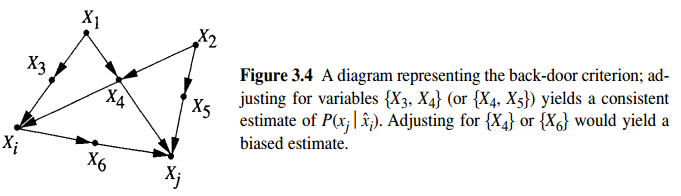
\includegraphics[scale = 0.6]{backdoor.png}}
\end{minipage}
\caption{\footnotesize{\textbf{The back-door adjustment  \citep{pearl2000causal}}}}
\label{fig: backdoor}
\end{figure}

\begin{itemize}
\item 
\begin{definition}(\textbf{\emph{Back-Door}}) \citep{pearl2000causal}\\
A set of variables $Z$ satisfies the \emph{\textbf{back-door criterion}} relative to an \emph{\textbf{ordered}} pair of variables $(X_i \rightarrow X_j)$ in a DAG $\cG$ if:
\begin{enumerate}
\item \emph{\textbf{no}} node in $Z$ is a \emph{\textbf{descendant}} of $X_i$; and
\item $Z$ \emph{\textbf{blocks every path}} between $X_i$ and $X_j$ that contains an arrow \textbf{\emph{into}} $X_i$.
\end{enumerate}
Similarly, if $X$ and $Y$ are two \textbf{disjoint} subsets of nodes in $\cG$, then $Z$ is said to satisfy \textbf{\emph{the back-door criterion}} relative to $(X, Y)$ if it satisfies the criterion relative to \emph{any pair} $(X_i, X_j)$ such that $X_i \in X$ and $X_j \in Y$.
\end{definition} 

\item  Satisfying the back-door criterion makes $Z$ a \emph{\textbf{sufficient adjustment set}}. The main insight of the graphical approach to covariate adjustment is that the adjustment set must \textbf{block all \emph{noncausal} paths} \textbf{without blocking} any \emph{\textbf{causal}} paths between $X$ and $Y$. 

\item \begin{theorem} (\textbf{Back-Door Adjustment}) \citep{pearl2000causal, neal2020introduction}\\
If a set of variables $Z$ satisfies the back-door criterion relative to $(X, Y)$, then the causal effect of $X$ on $Y$ is \textbf{identifiable} and is given by the formula
\begin{align}
P(y\,|\, do(x)) &= \sum_{z}P(y\,|\,x,  z)P(z) \label{eqn: back_door_adjustment}
\end{align}
\end{theorem} To see why this works we need to know that $P(z| do(x)) = P(z)$ since by back-door criterion, $Z$ has no descendant of $X$. Also $P(y\,|\,do(x),  z) = P(y\,|\,x,  z)$ since $Z$ blocks all paths from $X$ to $Y$, so by modularity 

\item Back-door criterion is equivalent to the \emph{\textbf{conditional exchangeability / unconfoundedness}} assumption as in \citep{imbens2015causal}.

\item The back-door adjustment is useful \textbf{only when} the \emph{\textbf{causal DAG is available}}.
\end{itemize}

\subsection{The Front-door Adjustment}
\begin{figure}
\begin{minipage}[t]{0.5\linewidth}
  \centering
  \centerline{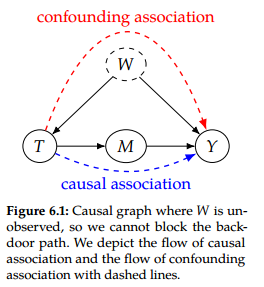
\includegraphics[scale = 0.6]{front_door_1.png}}
  \vspace{-5pt}
  \centerline{(a)}
\end{minipage}
\begin{minipage}[t]{0.5\linewidth}
  \centering
  \centerline{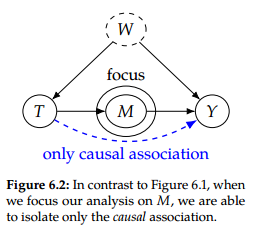
\includegraphics[scale = 0.6]{front_door_2.png}}
  \vspace{-5pt}
  \centerline{(b)}
\end{minipage}\\
\begin{minipage}[t]{0.5\linewidth}
  \centering
  \centerline{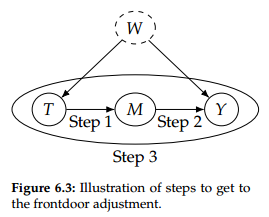
\includegraphics[scale = 0.6]{front_door_3.png}}
  \vspace{-5pt}
  \centerline{(c)}
\end{minipage}
\caption{\footnotesize{\textbf{The front-door adjustment when the covariates in back-door path is not observed. }}}
\label{fig: front_door}
\end{figure}
\begin{itemize}
\item The back-door criterion provides \emph{\textbf{sufficient condition}} to identify adjustment set. If the covariates in back-door path is unobserved, it is not possible to block back-door path. Figure \ref{fig: front_door} (a). 

\item If there exists a \emph{\textbf{mediator}} $M$ in the path from $T$ to $Y$ (i.e. $T\rightarrow M \rightarrow Y$), we can isolate the association that flows through $M$ by focusing our statistical analysis on $M$, and the only association that flows through $M$ is causal association.

\item We will focus our analysis on $M$ using a \textbf{three step procedure} (see Figure \ref{fig: front_door} (c) for our corresponding illustration):
\begin{enumerate}
\item \textbf{Identify the causal effect of $T$ on $M$, i.e. $\underline{p(m|\,do(t))}$.} From Figure \ref{fig: front_door} (b), we see that $M\rightarrow Y \leftarrow W$, i.e. $Y$ is a collider between $W$ and $M$. This means that the back-door path to $T$ from $M$ is blocked. So $T$ satisfies back-door criterion and $T\rightarrow M$ is a causal association. Thus the adjustment set is empty and by back-door adjustment
\begin{align*}
p(m|\, do(t)) &= p(m|\, t)
\end{align*} 
\item \textbf{Identify the causal effect of $M$ on $Y$, i.e. compute $\underline{p(y |\, do(m))}$.} Because $T$ blocks the backdoor path $Y\leftarrow W \rightarrow T \rightarrow M$, we can simply adjust for $T$. Using back-door adjustment
\begin{align*}
p(y | \, do(m)) &= \sum_{t'}p(y|\, m, t')\,p(t')
\end{align*}

\item \textbf{Combine the above steps to identify the causal effect of $T$ on $Y$.}
\begin{align*}
p(y | \, do(t)) &= \sum_{m} \,p(m|\, do(t))\, p(y | \, do(m))  \\
&= \sum_{m}p(m|\, t)\,\sum_{t'}p(y|\, m, t')\,p(t')
\end{align*} The first factor on the right-hand side corresponds to setting $T$ to $t$ and observing the resulting value of $M$. The second factor corresponds
to \textbf{setting} $M$ to \textbf{exactly} the value $m$ that \textbf{resulted from setting} $T$ and then observing what value of $Y$ results. 
\end{enumerate}

\item \begin{definition} (\emph{\textbf{Front-Door}}) \citep{pearl2000causal}\\
A set of variables $M$ is said to satisfy the \emph{\textbf{front-door criterion}} relative to an \emph{\textbf{ordered}} pair of variables $(T, Y)$ if:
\begin{enumerate}
\item $M$ \textbf{intercepts} \textbf{all} directed paths from $T$ to $Y$;
\item there is \emph{\textbf{no unblocked back-door path}} from $T$ to $M$; and
\item \emph{\textbf{all back-door paths}} from $M$ to $Y$ are \emph{\textbf{blocked}} by $T$.
\end{enumerate}
\end{definition} 

\item  A set of variables $M$ \emph{\textbf{completely mediates}} the effect of $T$ on $Y$ if all causal (directed) paths from $T$ to $Y$ go through $M$. If $M$ satisfies the front-door criterion, $M$ is a set of complete mediators.

\item \begin{theorem}(\textbf{Front-Door Adjustment}) \citep{pearl2000causal, neal2020introduction}\\
If $M$ satisfies the front-door criterion relative to $(T, Y)$ and if $P(t, m) > 0$, then the causal
effect of $T$ on $Y$ is \textbf{identifiable} and is given by the formula
\begin{align}
P(y | \, do(t)) &=  \sum_{m}P(m|\, t)\,\sum_{t'}P(y|\, m, t')\,\,P(t')
\end{align}
\end{theorem}
\begin{proof}
We can prove this theorm using Rules from \emph{do}-calculus.
\begin{align*}
P(y | \, do(t)) &= \sum_{m} P(y | \, do(t), m) P(m |\, do(t)) \quad (\text{marginalization trick})\\
&= \sum_{m} P(y | \, do(t), m) P(m |\, t) \quad \text{(\textbf{action to observation on $t$})}\\
&=  \sum_{m} P(y | \, do(t), do(m)) P(m |\, t) \quad \text{(\textbf{observation to action exchange on $m$})}\\
&= \sum_{m} P(y | \, do(m)) P(m |\, t) \quad \text{(\textbf{deletion of actions $do(t)$})} \\
&= \sum_{m} P(m |\, t) \sum_{t'} P(y | \, do(m), t')\, p(t' |\, do(m)) \quad (\text{marginalization trick}) \quad  \\
&= \sum_{m} P(m |\, t) \sum_{t'} P(y | \, m,  t')\, p(t' |\, do(m))  \quad \text{(\textbf{action to observation on $m$})} \\
&= \sum_{m} P(m |\, t) \sum_{t'} P(y | \, m,  t')\, p(t')  \quad \text{(\textbf{deletion of actions $do(m)$})} \qed
\end{align*} 
\begin{itemize}
\item  Because the backdoor path from $T$ to $M$ is blocked by the collider $Y$, all of the association that flows from $T$ to $M$ is causal. Thus $P(m |\, do(t)) = P(m |\, t)$

\item Under $do(T=t)$, there is no back-door path from $M$ to $T$ in induced graph. So $P(y | \, do(t), m) = P(y | \, do(t), do(m))$.

\item Note that $M$ is a fully mediator. Given $do(M=m)$, we can remove the link between $T$ to $M$ and $Y \indep T | M$ in the induced graph. Thus we drop $do(T=t)$. 

\item We then introduce $T$ by conditioning and marginalizing on $T$.  Given $T=t'$,  $T$ blocks all back-door from $M$ to $Y$ so $M\rightarrow T$ is causal link, i.e. $P(y | \, do(m), t') = P(y | \,m, t')$

\item Finally, $M$ has no causal effect on $T$ since the back-door path is blocked by $Y$. So $p(t' |\, do(m)) = p(t')$.
\end{itemize}
\end{proof}

\end{itemize}

\subsection{Propensity scores}
\begin{itemize}
\item Given a high dimensional confounder set $W$ that satisfies the backdoor criterion (or, equivalently, that $T \indep Y | W$),  it is not necessary to control on all of covariates in $W$. 

\begin{figure}
\begin{minipage}[t]{1\linewidth}
  \centering
  \centerline{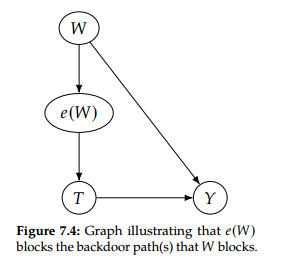
\includegraphics[scale = 0.6]{propensity_score.png}}
\end{minipage}
\caption{\footnotesize{\textbf{The propensity score blocks the backdoor paths  \citep{neal2020introduction}}}}
\label{fig: propensity_score}
\end{figure}


\item 
\begin{definition} (\emph{\textbf{Propensity Scores}}) \citep{rosenbaum2017observation, neal2020introduction}\\
If $W$ satisfies \emph{\textbf{unconfoundedness}} and \emph{\textbf{positivity}}, the \underline{\emph{\textbf{propensity score}}} is defined as
\begin{align}
e(W) &= P(T=1 \,|\, W). \label{eqn: propensity_score}
\end{align} It is the probabiilty of receiving treatment  \emph{\textbf{within levels of}} $W$.
\end{definition}

\item 
\begin{theorem} (\textbf{Propensity Score Theorem}) \citep{neal2020introduction}\\
Given positivity, unconfoundedness given $W$, implies \textbf{unconfoundedness} given the propensity score $e(W)$.
\begin{align}
(Y(1), Y(0)) \indep T \;|\; W \;\; \Rightarrow\;\; (Y(1), Y(0)) \indep T \;|\; e(W) \label{eqn: conditional_exchangeablity_propensity_score}
\end{align}
\end{theorem}

\item To prove this theorem, we note that $e(W)$ completely determines the edge $W\rightarrow T$, since it completely describes the mechanism $P(T|W)$ with binary $T\in \set{0,1}$. Thus we can think of the \emph{propensity score} as a \emph{\textbf{full mediator}} of the effect of $W$ on $T$. Figure \ref{fig: propensity_score} indicates that $(e(W))$ blocks the back-door path that $W$ blocks. Therefore, we have a graphical proof of the propensity score theorem using the backdoor adjustment.

\item Recall The \emph{\textbf{Positivity-Unconfoundedness Tradeoff}}. As  the dimensionality of $W$ increases, the confoundedness will decrease, but the propensity score $e(W)$ will decrease, since the \emph{\textbf{overlap}} between control and treatment group will decrease. This is also effect of \emph{\textbf{the curse of dimensionality}}.

\item The propensity score $e(W)$ is usually unknown and we need to estimate it by training a model (e.g. \emph{logistic regression}) to predict $T$ from $W$.  
\end{itemize}



\section{Controlling covariate balance by matching}
\begin{itemize}
\item A critical difference between randomized experiments and observational studies is that the covariate balance is not guaranteed in observation study. It puts in question the comparablity between treatment and control groups. 

\item In order to obtain covariate balance, we can select sub-populations of treatments and control group so that their (observed) covariate distributions are close (\emph{\textbf{stochastic balancing}}). This process is called \emph{\textbf{matching}} or \emph{\textbf{treatment selection}}. 

\item Matching is a naive approach to address the \emph{\textbf{comparability}} issue: it says that people who \emph{look comparable} are comparable.

\item The \textbf{advantages} for matching include:
\begin{itemize}
\item \emph{\textbf{Controlling for confounder}} is achieved \textbf{at design phase} \emph{without looking at outcomes}. 

\item Matching will reveal \emph{\textbf{lack of overlap}} in \emph{covariate distribution}. That is, matching guarantees that the \textbf{\emph{positivity assumption}} holds for both control and treatment group.

\item Once matched, we can \textbf{treat it as randomized experiments}. 

\item Outcome analysis could be simple.
\end{itemize}

\item Usually we care about causal treatment effects \emph{\textbf{on the treated}} so we choose a subset of control group to \textbf{match the treatment group}.
\end{itemize}

\subsection{Matching directly on confounders}
\begin{itemize}
\item In order to find matches between treatment and control, we need to define some distance metrics to define \emph{closeness}. 
\begin{enumerate}
\item The \emph{\textbf{Mahalanobis distances}} between covariate of $i$, $\mb{w}_i$ and covariate of $j$, $\mb{w}_j$ is
\begin{align*}
d_{\mb{\Sigma}}(\mb{w}_i, \mb{w}_j) &= \paren{\paren{\mb{w}_i-\mb{w}_j}^{T}\mb{\Sigma}^{-1}\paren{\mb{w}_i-\mb{w}_j}}^{\frac{1}{2}}
\end{align*} for some positive definite matrix $\mb{\Sigma}$. A common choice of $\mb{\Sigma} = \widehat{\text{Cov}}(W)$ is the estimated \textbf{covariance matrix} for $W$.

\item The \emph{\textbf{Robust Mahalanobis distances}} \citep{rosenbaum2017observation} is proposed to handle \textbf{outliers} in the covariates to avoid they increase the distance too much while the other covariates remain close. 

The idea to use \emph{\textbf{order statistics (ranks)}} instead of absolute values for each $\mb{w}_{i}$.
\begin{align*}
d_{robust}(\mb{w}_i, \mb{w}_j) &= \norm{\mb{r}(\mb{w}_{i}) -  \mb{r}(\mb{w}_{j})}{2}
\end{align*} where $\mb{r}(\mb{w}) = [r(w_1), \ldots, r(w_{k})]$ is a list of ranks for each covariate.

\item The distance between \emph{\textbf{propensity scores}} $d_{e}(\mb{w}_i, \mb{w}_j) := \norm{e(\mb{w}_i) - e(\mb{w}_j)}{2}$.
\end{enumerate}

\item During \underline{\emph{\textbf{pair matching (i.e. one-to-one matching)}}}, we select subject $i$ with $\mb{w}_{i}$ \emph{in the control group} whose distance $d(\mb{w}_i, \mb{w}_r) \le \epsilon$ for some $\epsilon >0$, where $\mb{w}_r$ corresponds to a reference subject $r$ in the treatment group. 
\end{itemize}

\subsection{Greedy matching by nearest neighbor}
\begin{itemize}
\item Instead of matching using fixed threshold $\epsilon$ ($\epsilon$-ball matching), we can determine the definition of closeness in nonparametric way.

\item \begin{definition} (\emph{\textbf{Nearest neighbor matching (Greedy matching)}})\\
Assume that $W$ is a \emph{\textbf{sufficient adjustment set}} that satisfies back-door criterion, i.e. the conditional ignorablity holds given $W$. Let $d_{i,j}:= d(\mb{w}_i, \mb{w}_{j})$, for $\mb{w}_i, \mb{w}_{j}\in W$ be pairwise distance between covariates of subjects in treatment and control groups. 

The \emph{\textbf{nearest neighbor matching}} (\emph{\textbf{greedy matching}}) has the following steps:
\begin{enumerate}
\item Randomly order list of subjects in control set $C$ and treatment set $T$;
\item (\textbf{Greedy match}) Select a treated subject $r \in T$. Choose a control subject $i \in C$ so that 
\begin{align*}
i &\in \arg\min_{j \in C} d(\mb{w}_r, \mb{w}_{j});
\end{align*} 

\item Remove matched control $i$ from $C$, i.e. $C \leftarrow C - \set{i}$ and $T \leftarrow T - \set{r}$;
\item Loop above steps until $T = \emptyset$ assuming more controls than treatments $|C| > |T|$. 
\end{enumerate}
\end{definition}

\item The benefits for greedy match are
\begin{enumerate}
\item \textbf{Intutive}. 
\item \textbf{Computational fast} if implemented with fast approximate nearest neighbor algorithms, locality sensitive hashing etc.
\end{enumerate}

\item On the other hand, the disadvantages are
\begin{enumerate}
\item \textbf{Not invariant to initial ordering}. Note that the previous match will affect the latter match since it will take out the candidates.  
\item \textbf{Not optimal}. It is a greedy algorithm, i.e. it does not guarantee that the closest distance match locally is the closest distance match globally. This is because this algorithm use \emph{\textbf{hard match assignment}} instead of \emph{soft match assignement} (i.e. with probability).
\end{enumerate}

\item An alternative to pair matching is \underline{\textbf{\emph{many-to-one matching ($k:1$ matching)}}}: after every one has $1$ match, we loop back to the first treated in the list and find the second best match of it. Loop until every one has exactly $k$ matches. 

\item There are several \textbf{tradeoffs} (\textbf{Bias-variance tradeoff}):
\begin{itemize}
\item  For pair matching, the matching is closer, thus has \textbf{low bias}, but have high variance and \textbf{less data efficient} since we are dropping data. It also has higher \textbf{computational speed}; 
\item  For many-to-one matching, it has \textbf{larger sample size} so it has smaller variance. It will add more bias since we are not selecting the best matches.
\end{itemize}

\item We might want to discard treated subjects when there is no good match. We referred to the \emph{\textbf{maximum acceptable distance}} as  a \emph{\textbf{caliper}} \citep{rosenbaum2017observation}.
\begin{itemize}
\item Only match a treated subject if the best match has distance less than the caliper. 
\item If no match within caliper, then the \textbf{positivity assumption} would be violated. Excluding these subjects makes the positivity assumption more realistic.
\item The drawback is that the \textbf{definition} of population is \textbf{unclear} after removing treated subjects.
\end{itemize}
\end{itemize}

\subsection{Optimal pair matching}
\begin{itemize}
\item Greedy matching is not \emph{global optimal}, i.e. $\sum_{r}d(\mb{w}_r, \mb{w}_{nn(r)}) \neq \min_{\set{j_1, \ldots, j_T}}\sum_{r}d(\mb{w}_r, \mb{w}_{j_r})$.

\item In optimal pair matching, the objective is to pairs $(r, j_r)$ for all $r \in T$ and $j_r \in C$ so that
\begin{align*}
\min_{\set{j_1, \ldots, j_T} \in C} &\sum_{r=1}^{T}d(\mb{w}_r, \mb{w}_{j_r}) 
\end{align*}

\item  It is  an \underline{\emph{\textbf{optimal assignment problem}}} \citep{gabriel2019computational}, where the pairwise distance is the cost for each pair assignment. This is also a \emph{\textbf{minimum flow problem}} in \textbf{network flow optimization} \citep{rosenbaum2017observation}. In particular, we can drop the integer constraint to obtain a \emph{linear programming relaxation} as
\begin{align*}
\min_{f(u, v) \, \forall (u,v) \in \cE_{C,T}}& d(\mb{w}_u, \mb{w}_{v}) f(u, v)\\
\text{s.t. }& \sum_{v \in \cV_{T}}f(u, v) = 1 \\
&\sum_{u \in \cV_{C}}f(u, v) =  1  \\
& f(u, v)  \ge 0, \quad \forall (u,v) \in \cE_{C,T}
\end{align*} where $\cG = (\cV_{C}\cup\cV_{T}, \cE_{C,T})$ is a bipartite graph between treatment and control group index set.

\item Whether or not it is feasible to perform optimal matching depends on the \textbf{size of the problem}. \textbf{Size} is typically measured by \emph{number of possible treatment-control pairing}, i.e. $|\cE_{C,T}|$.

\item Contraints can be imposed to make optimal matching computationally feasible for larger data set, i.e. reduce the edge set $\cE_{C,T}$. This is known as \emph{\textbf{sparse matching}}.
\end{itemize}

\subsection{Matching by propensity score}
\begin{itemize}
\item The propensity score $e(W)$ computes the probability of receiving treatment under levels of $W$.  In \emph{\textbf{completely randomized experiments}}, it is pre-determined $e(\mb{w}) = \frac{1}{2}$ for all $\mb{w}$.

\item If two subjects have the \textbf{same propensity score}, $e(\mb{w})$, they may have different values of $\mb{w}$. However, their effects on the treatment assignment $T$ is equal. 

%\item If subjects were matched for $e(\mb{w})$, they may be mismatched for $\mb{w}$, but the mismatches in $\mb{w}$ will be due to chance and will tend to balance, particularly in large samples.  In brief, \underline{\textbf{matching on $e(\mb{w})$ tends to balance $\mb{w}$}}.

\item The \emph{goal} is to choose the subpopulation with estimated propensity score $\hat{e}(\mb{w}_{n})$ \textbf{matches} between treatment and control groups.

 We can use distance-based matching as discussed above.

\item The \textbf{\emph{advantages}} of matching by propensity score:
\begin{itemize}
\item Matching on $e(\mb{w})$ is often \emph{\textbf{practical}} even when there are many covariates in $\mb{w}$ because $e(\mb{w})$  is a \textbf{single} variable;
\item \underline{\textbf{\emph{Matching on $e(\mb{w})$ tends to balance all of $\mb{w}$}}} (i.e. \emph{propensity score is a \textbf{matching score}});

Note that $e(W)$ is a full mediator of $W$ to $T$. So the covariate balance between control and treatment group given that the propensity score is matched.
\begin{align*}
W \indep T \,|\,e(W) \Leftrightarrow \quad p(W |\,e(W) = e,\, T= 0) = p(W |\,e(W) = e,\, T= 1)
\end{align*}

\item Failure to balance $e(\mb{w})$ implies that $\mb{w}$ is not balanced.
\end{itemize}

\item Given estimated propensity score, it is useful to first check the \textbf{overlap of support} for \textbf{propensity score distributions} $p(\hat{e}(W)| T)$ between treatment and control before matching. This is to verify the positivity assumption. 

\item If there lacks of overlap, \textbf{trimming the tails} is an option, i.e. to remove subjects with extreme scores. It would prevent \emph{\textbf{extrapolations}}. 

\item In practice, the \underline{\textbf{\emph{log-odds (logit) of propensity score}}} $\text{logit}(e(W)) := \log\paren{\frac{e(W)}{1- e(W)}}$ is often used as an alternative unbounded score which preserves ranks.

\item In practice, the \emph{\textbf{caliper}} is chosen as $0.2 \times \sigma\paren{\text{logit}(e(W))}$.

%\item Ignoring chance imbalances, as we might in sufficiently large samples, balancing the propensity score $e(\mb{w})$ is sufficient to balance the observed covariates $\mb{w}$ but also necessary to balance $\mb{w}$. 

\item It is important to understand that this is a true statement about \textbf{observed covariates} $\mb{w}$, and \textbf{only} about observed covariates, whether or not treatment assignment also depends on covariates that were \textbf{not measured}.

On the negative side, success in balancing the observed covariates, $\mb{w}$, provides \emph{\textbf{no assurance}} that \textbf{unmeasured covariates} are balanced  \citep{rosenbaum2017observation}.
\end{itemize}
\subsection{Accessing balance}
\begin{itemize}
\item After the matching is completed, we can evaluate its performance by checking on the covariate distributions for treatment and control groups.

\item Hypothesis testing (two-sample $t$-test) and make decision based on p-values. Note that p-value is determined by the sample size as well.

\item We can use a table that looks at pre-matching vs. post-matching covariate balance. In each part, we look at the \emph{\textbf{standardized mean differences}}
\begin{align*}
\text{smd} &= \frac{\bar{m}_{T} - \bar{m}_{C}}{\sqrt{\frac{\hat{\sigma}_{T}^{2} + \hat{\sigma}_{C}^{2}}{2}}}
\end{align*}

We can compute the standardized differences for each covariate. Usually choose threshold as $\le 0.1$.

\end{itemize}

\section{Unobserved Confounding}
\begin{itemize}
\item In observational studies, there could also be some \emph{\textbf{unobserved confounder(s)}}. Therefore, we’d like to know how \textbf{robust} our estimates are to unobserved confounding.
\begin{itemize}
\item The first way we can do is by getting an \emph{upper and lower \textbf{bound}} on the causal effect using credible \textbf{assumptions}.

\item Another way we can do this is by simulating \textbf{how strong} the confounder’s effect on the treatment and the confounder’s effect on the
outcome need to be to make \emph{the true causal effect \textbf{substantially different} from our estimate} (i.e. \emph{\textbf{sensitivity analysis}}).

\item We can also use the \textbf{\emph{instrumental variables}}, which will be discussed in its own chapter.
\end{itemize}
\end{itemize}
\subsection{Bounds}
\begin{itemize}
\item Depending on what assumptions we are willing to make, we can derive various nonparametric bounds on causal effects. For example, the unconfoundedness assumption before might be unrealistic given unobserved confounder exists. In this section, we use assumptions weaker than the unconfoundedness assumption.

\item Rather than telling us exactly what the causal effect must be, we can give \textbf{an interval} that the causal effect must be in. 

\item Under the unconfoundedness assumption, the interval will collapse to be a single point.  
\end{itemize}

\subsubsection{No-assumptions bound}
\begin{itemize}
\item \begin{assumption} (\textbf{Bounded Potential Outcomes}) \citep{neal2020introduction}\\
\begin{align}
a \le Y(0), Y(1) \le b \label{eqn: bounded_potential_assumption}
\end{align}
\end{assumption}

\item We can find a decomposition of the \textbf{Average Treatment Effect (ATE)}
\begin{proposition} (\textbf{Observational-Counterfactual Decomposition})  \citep{neal2020introduction}\\
\begin{align}
\E{}{Y(1) - Y(0)} &= \set{\pi\, \E{}{Y \,|\, T = 1} - (1-\pi)\, \E{}{Y\,|\, T=0}}   \nonumber\\
&\quad +  \set{(1-\pi)\, \E{}{Y(1) \,|\, T=0 } - \pi\, \E{}{Y(0) \,|\, T=1} }  \label{eqn: ate_obs_count_decomp}
\end{align} where $\pi = P(T=1)$.
\end{proposition}
\begin{proof}
Note 
\begin{align*}
\E{}{Y(1) - Y(0)} &=p(T=1) \E{}{Y(1) - Y(0) | T=1} + p(T=0) \E{}{Y(1) - Y(0) | T=0} \\
 &= \pi \E{}{Y(1)\,| \, T=1} - \pi \E{}{Y(0) | T=1}  \nonumber \\
 &\quad +(1-\pi)\E{}{Y(1) \,|\, T=0}  -  (1-\pi)\E{}{Y(0) \,|\, T=0} \\
 &=  \pi \E{}{Y\,| \, T=1}   - \pi \E{}{Y(0) | T=1} \quad\text{ (by consistency)}  \nonumber \\
 &\quad +(1-\pi)\E{}{Y(1) \,|\, T=0}  -  (1-\pi)\E{}{Y \,|\, T=0} \qed
\end{align*} 
\end{proof}

\item The first two terms in \eqref{eqn: ate_obs_count_decomp} are \emph{\textbf{observational}} and the last two term are \emph{\textbf{counterfactual}}. Since the last two terms are not observed, we need to bound the difference using bounded potential outcome assumption \eqref{eqn: bounded_potential_assumption}.

\item \begin{proposition} (\textbf{No-Assumptions Bound})  \citep{neal2020introduction}\\
Let $\pi$ denote $P(T = 1)$, where $T$ is a binary random variable. Given that the outcome $Y$ is bounded between $a$ and $b$ (Assumption 4.1), we have the following \textbf{upper and lower bounds} on the ATE:
\begin{align}
\E{}{Y(1) - Y(0)} \le \set{\pi\, \E{}{Y \,|\, T = 1} - (1-\pi)\, \E{}{Y\,|\, T = 0\,}} + \brac{(1-\pi)\,b - \pi \,a} \label{eqn: no_assumption_upper_bound}\\
\E{}{Y(1) - Y(0)} \ge \set{\pi\, \E{}{Y \,|\, T = 1} - (1-\pi)\, \E{}{Y\,|\, T = 0\,}} + \brac{(1-\pi)\,a - \pi \,b} \label{eqn: no_assumption_lower_bound}
\end{align} More importantly, the interval where $\E{}{Y(1) - Y(0)}$ lies has length $(b-a) / 2$.
\end{proposition}

\end{itemize}
\subsubsection{Monotone treatment response}
\begin{itemize}
\item In order to improve the no-assumption bounds, we need to consider additional assumptions on the counterfactual difference terms  in \eqref{eqn: ate_obs_count_decomp}.

\item \begin{assumption} (\textbf{Nonnegative Monotone Treatment Response}) \citep{neal2020introduction}\\
\begin{align}
\forall\,i,\quad Y_i(1) \ge Y_i(0). \label{eqn: nonnegative_mtr_assumption}
\end{align}
\end{assumption}

\item This means that every ITE is nonnegative, i.e. \emph{\textbf{the treatment cannot hurt anyone}}. It is easy to see that the ATE is above zero. This can be derived by seeing 
\begin{align*}
\E{}{Y(1) \,|\, T=0}  &\ge \E{}{Y(0) | T=0} = \E{}{Y | T=0} \\
-\E{}{Y(0) | T=1} &\ge- \E{}{Y(1)\,| \, T=1}  =  -\E{}{Y\,| \, T=1}   
\end{align*} Substituting this into \eqref{eqn: ate_obs_count_decomp}, we can have the bound

\item \begin{proposition} (\textbf{Nonnegative MTR Lower Bound})  \citep{neal2020introduction}\\
Under the nonnegative MTR assumption, the ATE is bounded from below by 0. Mathematically,
\begin{align*}
\E{}{Y(1) - Y(0)}  \ge 0
\end{align*}
\end{proposition}

\item We can switch the sign if we have \emph{Nonpositive Monotone Treatment Response}.
\end{itemize}
\subsubsection{Monotone treatment selection}
\begin{itemize}
\item \begin{assumption} (\textbf{Monotone Treatment Selection}) \citep{neal2020introduction} \\
\begin{align}
\E{}{Y(1) \,|\, T=1}  &\ge \E{}{Y(1) \,|\, T=0} \nonumber\\
\E{}{Y(0) \,|\, T=1}  &\ge \E{}{Y(0) \,|\, T=0} \label{eqn: mts_assumption}
\end{align}
\end{assumption}

\item This assumes that the people who \textbf{\textbf{selected treatment}} would have \textbf{better outcomes} than those who didn’t select treatment, under either treatment scenario.  

\item \begin{proposition} (\textbf{Monotone Treatment Selection Upper Bound})  \citep{neal2020introduction}\\
Under the MTS assumption, the ATE is bounded from above by the \textbf{associational difference}. Mathematically,
\begin{align}
\E{}{Y(1) - Y(0)}  &\le \E{}{Y\,|\, T = 1} -  \E{}{Y\,|\, T = 0}  \label{eqn: mts_upper_bound}
\end{align}
\end{proposition}
\begin{proof}
\begin{align*}
\E{}{Y(1) - Y(0)}  &=  \set{\pi\, \E{}{Y \,|\, T = 1} - (1-\pi)\, \E{}{Y\,|\, T=0}}   \nonumber\\
&\quad +  \set{(1-\pi)\, \E{}{Y(1) \,|\, T=0 } - \pi\, \E{}{Y(0) \,|\, T=1} } \\
&\le  \set{\pi\, \E{}{Y \,|\, T = 1} - (1-\pi)\, \E{}{Y\,|\, T=0}}   \nonumber\\
&\quad +  \set{(1-\pi)\, \E{}{Y(1) \,|\, T=1 } - \pi\, \E{}{Y(0) \,|\, T=0} } \\
&= \E{}{Y \,|\, T = 1} - \E{}{Y\,|\, T=0} \qed
\end{align*}
\end{proof}
\end{itemize}
\subsubsection{Optimal treatment selection}
\begin{itemize}
\item \begin{assumption} (\textbf{Optimal Treatment Selection}) \citep{neal2020introduction} \\
\begin{align}
T_i = 1 \Rightarrow Y_i(1) \ge Y_i(0), &\quad \text{and } \quad T_i = 0 \Rightarrow Y_i(0) > Y_i(1)  \label{eqn: ots_assumption}
\end{align}
\end{assumption}

\item This assumption means that the individuals always receive the treatment that is \textbf{best} for them (e.g. if an expert doctor is deciding which treatment to give people).

\item From OTS, we see that 
\begin{align*}
\E{}{Y(0) \,|\, T=1} &\le \E{}{Y(1) \,|\, T=1} = \E{}{Y \,|\, T=1} \\
\E{}{Y(1) \,|\, T=0} &< \E{}{Y(0) \,|\, T=0} = \E{}{Y \,|\, T=0}.
\end{align*} We can combine OTS and bounded potential outcomes to have new bound

\item \begin{proposition} (\textbf{Optimal Treatment Selection Bound 1}) \citep{neal2020introduction} \\
Let $\pi$ denote $P(T = 1)$, where $T$ is a binary random variable. Given that the outcome $Y$ is bounded from below by $a$ (Assumption 4.1) and that the optimal treatment is always selection (Assumption 4.8), we have the following upper and lower bounds on the ATE:
\begin{align}
\E{}{Y(1) - Y(0)}  &< \pi \E{}{Y \,|\, T=1} - \pi \,a \label{eqn: ots_upper_bound_1} \\
\E{}{Y(1) - Y(0)}  &\ge (1-\pi)\,a - (1-\pi) \E{}{Y \,|\, T=0}  \label{eqn: ots_lower_bound_1} \\
(\text{Interval Length}) &= \pi \E{}{Y \,|\, T=1} + (1-\pi) \E{}{Y \,|\, T=0} - a \label{eqn: ots_int_len_1}
\end{align}
\end{proposition}

\item From the OTS, we can also derive
\begin{align}
\E{}{Y(1) \,|\, T = 0} &= \E{}{Y(1)\, |\, Y(0) > Y(1)} \quad (\text{by OTS}) \nonumber\\
&  <  \E{}{Y(1)\, |\, Y(0) \le Y(1)} \nonumber\\
& \quad \text{since }  \E{}{Y(1)\, |\, Y(0) > Y(1)} < \E{}{Y(0)} \le \E{}{Y(1)\, |\, Y(1) \ge Y(0) } \nonumber\\
&= \E{}{Y(1)\, |\, T = 1}   \quad (\text{by counterpositive argument of OTS}) \nonumber\\
&= \E{}{Y\, |\, T = 1} \label{eqn: ots_counter_upper_bound}
\end{align} In other word, the \textbf{counterfactual outcome} \underline{\emph{\textbf{given not treated}}} will still be \emph{\textbf{worse}} than the \textbf{actual outcome} \underline{\emph{\textbf{given treated}}}. (actual outcome better than speculated outcome)

Substitute this bound to \eqref{eqn: ate_obs_count_decomp}, we have the following bound

\item \begin{proposition} (\textbf{Optimal Treatment Selection Bound 2}) \citep{neal2020introduction} \\
Let $\pi$ denote $P(T = 1)$, where $T$ is a binary random variable. Given that the outcome $Y$ is bounded from below by $a$ (Assumption 4.1) and that the optimal treatment is always selection (Assumption 4.8), we have the following upper and lower bounds on the ATE:
\begin{align}
\E{}{Y(1) - Y(0)}  &< \E{}{Y \,|\, T=1} - \pi \,a - (1-\pi) \E{}{Y\,|\, T=0} \label{eqn: ots_upper_bound_2} \\
\E{}{Y(1) - Y(0)}  &\ge \pi \E{}{Y \,|\, T=1}+ (1-\pi)\,a -  \E{}{Y \,|\, T=0}  \label{eqn: ots_lower_bound_2} \\
(\text{Interval Length}) &= (1-\pi) \E{}{Y \,|\, T=1} + \pi \E{}{Y \,|\, T=0} - a \label{eqn: ots_int_len_2}
\end{align}
\end{proposition}

This interval \eqref{eqn: ots_int_len_2} is usually larger than that in \eqref{eqn: ots_int_len_1}. But the lower bound can be above zero. And we can take intersection between the intervals from OTS bound 1 and bound 2.

\item Some important takeaways:
\begin{itemize}
\item Different bounds are better in \textbf{different cases}.
\item Different bounds can be better in different ways (e.g., \emph{identifying the sign} vs. getting \emph{a smaller interval}).
\end{itemize}

\end{itemize}
\subsection{Sensitivity analysis}
\subsubsection{Overview}
\begin{itemize}
\item Matching aims to achieve covariate balance on \emph{observed covariates}. If there was imbalance on observed covariates, we have \textbf{overt bias} (i.e. we do not have full control over these covariates). 

\item When the  \textbf{\emph{unobserved confounder}}  exists, we have \underline{\textbf{\emph{hidden bias}}}. In
this situtation, the causal effect is \emph{\textbf{not identifiable}}.

\item The \textbf{main idea} of \underline{\emph{\textbf{sensitivity analysis}}} is to determine how severe the hidden bias has to be in order to \textbf{change the conclusion} e.g. change the \emph{statistical significance} of the results or change the \emph{direction} of effect.
\end{itemize}
\subsubsection{Sensitivity basics in linear setting}
\begin{figure}
\begin{minipage}[t]{1\linewidth}
  \centering
  \centerline{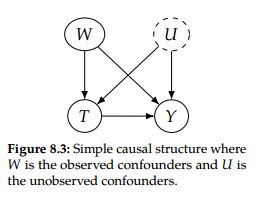
\includegraphics[scale = 0.7]{scm_sensitivity.png}}
\end{minipage}
\caption{\footnotesize{\textbf{The linear structural equations with an unobserved confounder $U$ for sensitivity analysis  \citep{neal2020introduction}}}}
\label{fig: scm_sensitivity}
\end{figure}

\begin{itemize}
\item Assume a \emph{\textbf{noiseless}} \emph{\textbf{linear}} structrual causal equation:
\begin{align}
T &:= \alpha_{w} W +  \alpha_u U  \label{eqn: sensitivity_analysis_scm_treatment}\\
Y &:= \beta_{w} W +  \beta_u U + \delta\,T \label{eqn: sensitivity_analysis_scm_effect}
\end{align} where $W$ and $U$ are both confounders for the causal effect of $T$ on $Y$. See Figure \ref{fig: scm_sensitivity}.

\item From this equation, we see that the ATE is determined by $\delta$. By back-door assignment, 
\begin{align*}
P(Y |\, do(T=t)\,) &= \sum_{w, u}P(Y \,|\, T=t, w, \, u)P(w, u) \\
\Rightarrow \E{}{Y(1) - Y(0)}  &=  \E{}{Y|\,do(T=1)\,} - \E{}{Y|\,do(T=0)\,} \\
&= \E{W, U}{\E{}{Y \,|\, T=1, W, U} - \E{}{Y \,|\, T=0, W, U}} = \delta
\end{align*}

\item But because $U$ isn’t observed, the best we can do is adjust for only $W$. This leads to a \emph{\textbf{confounding bias (hidden bias)}} of $\frac{\beta_{u}}{\alpha_u}$

\item \begin{proposition}  \citep{neal2020introduction} \\
 When $T$ and $U$ are generated by the \textbf{noiseless linear process} in Equations \eqref{eqn: sensitivity_analysis_scm_treatment} and \eqref{eqn: sensitivity_analysis_scm_effect}, the \textbf{confounding bias} of adjusting for \textbf{just} $W$ (and not $U$) is $\frac{\beta_{u}}{\alpha_u}$. Mathematically:
 \begin{align}
 &\E{W}{\E{}{Y \,|\, T=1, W} - \E{}{Y \,|\, T=0, W}} \nonumber\\
 &-  \E{W, U}{\E{}{Y \,|\, T=1, W, U} - \E{}{Y \,|\, T=0, W, U}} = \frac{\beta_{u}}{\alpha_u} \label{eqn: sensitivity_analysis_linear}
 \end{align}
 \end{proposition}
 \begin{proof}
 We’ll prove Proposition  in 3 steps:
 \begin{enumerate}
 \item Get a closed-form expression for $\E{W}{\E{}{Y \,|\, T=t, W}}$ in terms of
$\alpha_{w}$, $\alpha_u$, $\beta_w$ and $\beta_u$.

\item Use step 1 to get a closed-form expression for the difference
$\E{W}{\E{}{Y \,|\, T=1, W} - \E{}{Y \,|\, T=0, W}}$

\item Subtract off $\E{W, U}{\E{}{Y \,|\, T=1, W, U} - \E{}{Y \,|\, T=0, W, U}} = \delta$
 \end{enumerate}
 
 The first step can be obtained by substituting the SCM  \eqref{eqn: sensitivity_analysis_scm_effect}.
 \begin{align}
 \E{W}{\E{}{Y \,|\, T=t, W}} &= \E{W}{\E{}{\beta_{w} W +  \beta_u U + \delta\,T \,|\, T=t, W}} \nonumber \\
 &= \E{W}{\beta_{w}W + \delta\,t + \beta_u \E{}{U \,|\, T=t, W}  }  \label{eqn: sensitivity_analysis_linea_proof_1}
 \end{align} From \eqref{eqn: sensitivity_analysis_scm_treatment}, we have 
 \begin{align}
 U &= \frac{T - \alpha_w\, W}{\alpha_{u}}.  \label{eqn: sensitivity_analysis_linea_proof_2}
 \end{align} So substituting it into \eqref{eqn: sensitivity_analysis_linea_proof_1}, we have
 \begin{align}
 \E{W}{\E{}{Y \,|\, T=t, W}} &=  \E{W}{\beta_{w}W + \delta\,t + \beta_u  \frac{t - \alpha_w\, W}{\alpha_{u}}  }  \nonumber\\
 &= \paren{\delta+ \frac{\beta_u}{\alpha_u} }\,t + \paren{\beta_w - \frac{\beta_u\,\alpha_w}{\alpha_u}}\E{}{W}   \label{eqn: sensitivity_analysis_linea_proof_3}
 \end{align}
 
 In the second step, substituting \eqref{eqn: sensitivity_analysis_linea_proof_3} into difference equation
 \begin{align}
 \E{W}{\E{}{Y \,|\, T=1, W}} - \E{W}{\E{}{Y \,|\, T=0, W}} &= \paren{\delta+ \frac{\beta_u}{\alpha_u} }  \label{eqn: sensitivity_analysis_linea_proof_4}
 \end{align}
 
 Finally, substracting $\E{W, U}{\E{}{Y \,|\, T=1, W, U} - \E{}{Y \,|\, T=0, W, U}} = \delta$, 
 \begin{align*}
  \E{W}{\E{}{Y \,|\, T=1, W}} - \E{W}{\E{}{Y \,|\, T=0, W}} - \E{W, U}{\E{}{Y \,|\, T=1, W, U} - \E{}{Y \,|\, T=0, W, U}} = \frac{\beta_u}{\alpha_u}
 \end{align*} \qed
 \end{proof}
 
\end{itemize}
\subsubsection{Sensitivity contour plots}

\begin{figure}
\begin{minipage}[t]{1\linewidth}
  \centering
  \centerline{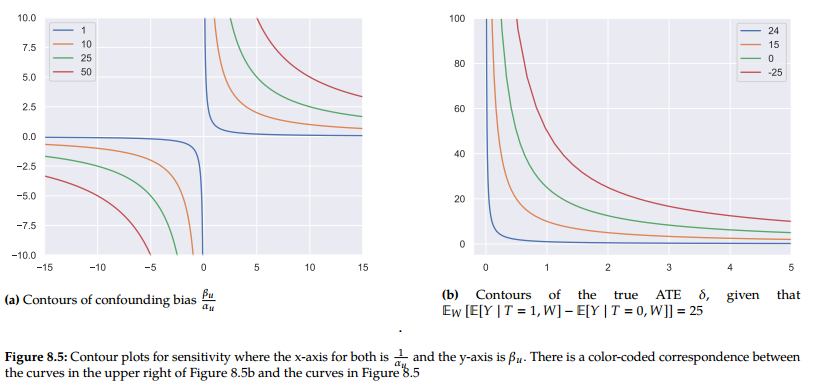
\includegraphics[scale = 0.55]{sensitivity_curve.png}}
\end{minipage}
\caption{\footnotesize{\textbf{The sensitivity curve for $\frac{\beta_u}{\alpha_u}$ under different choice of  $(\alpha_u, \beta_u)$  \citep{neal2020introduction}}}}
\label{fig: sensitivity_curve}
\end{figure}

\begin{itemize}
\item  We can rearrange the equation \eqref{eqn: sensitivity_analysis_linear} 
 \begin{align*}
 \delta &=  \E{W}{\E{}{Y \,|\, T=1, W} - \E{}{Y \,|\, T=0, W}} -  \frac{\beta_u}{\alpha_u} 
 \end{align*}

Thus so for given values of $\alpha_u$ and $\beta_u$, we can compute the \textbf{true ATE} $\delta$, from the \emph{observational quantity} $\E{W}{\E{}{Y \,|\, T=1, W} - \E{}{Y \,|\, T=0, W}}$

\item This allows us to get \textbf{\emph{sensitivity curves}} that allow us to know how \underline{\textbf{\emph{robust}}} conclusions like "$\E{W}{\E{}{Y \,|\, T=1, W} - \E{}{Y \,|\, T=0, W}} = 25$ is positive, so $\delta$ is likely positive"  are to \emph{unobserved confounding}. See Figure \ref{fig: sensitivity_curve}.

\item In other word, the observed quantity $\E{W}{\E{}{Y \,|\, T=1, W} - \E{}{Y \,|\, T=0, W}}$ need to be \emph{at least}  $\frac{\beta_u}{\alpha_u}$ in order to \emph{\textbf{change the sign}} of ATE. 

\item Note that $\alpha_u$ describes the \textbf{strength of influence} for the \emph{unobserved confounder} $U$ on \textbf{treatment} $T$ and $\beta_u$ describes the \textbf{strength of influence} for $U$ on \textbf{outcome} $Y$. 
\begin{align*}
\text{Confounding bias} =  \frac{\beta_u}{\alpha_u} = \frac{\text{strength}(U \rightarrow Y)}{\text{strength}(U \rightarrow T)}
\end{align*}
Thus \textbf{confounding bias}, i.e. the gap $\frac{\beta_u}{\alpha_u}$ between ATE and the \emph{\textbf{associational difference}} by controlling \textbf{observed confounder} $W$ is \textbf{\emph{propotional}} to  the \emph{strength of influence} of unobserved confounder $U$ on \textbf{outcome} and \textbf{\emph{inversely propotional}} to the  \emph{strength of influence} of  $U$ on the \textbf{treatment} $T$.
\end{itemize}
\newpage
\bibliographystyle{plainnat}
\bibliography{book_reference.bib}
\end{document}